\newpage
\tikz[remember picture,overlay] \node[opacity=1,inner sep=0pt] at (current page.center){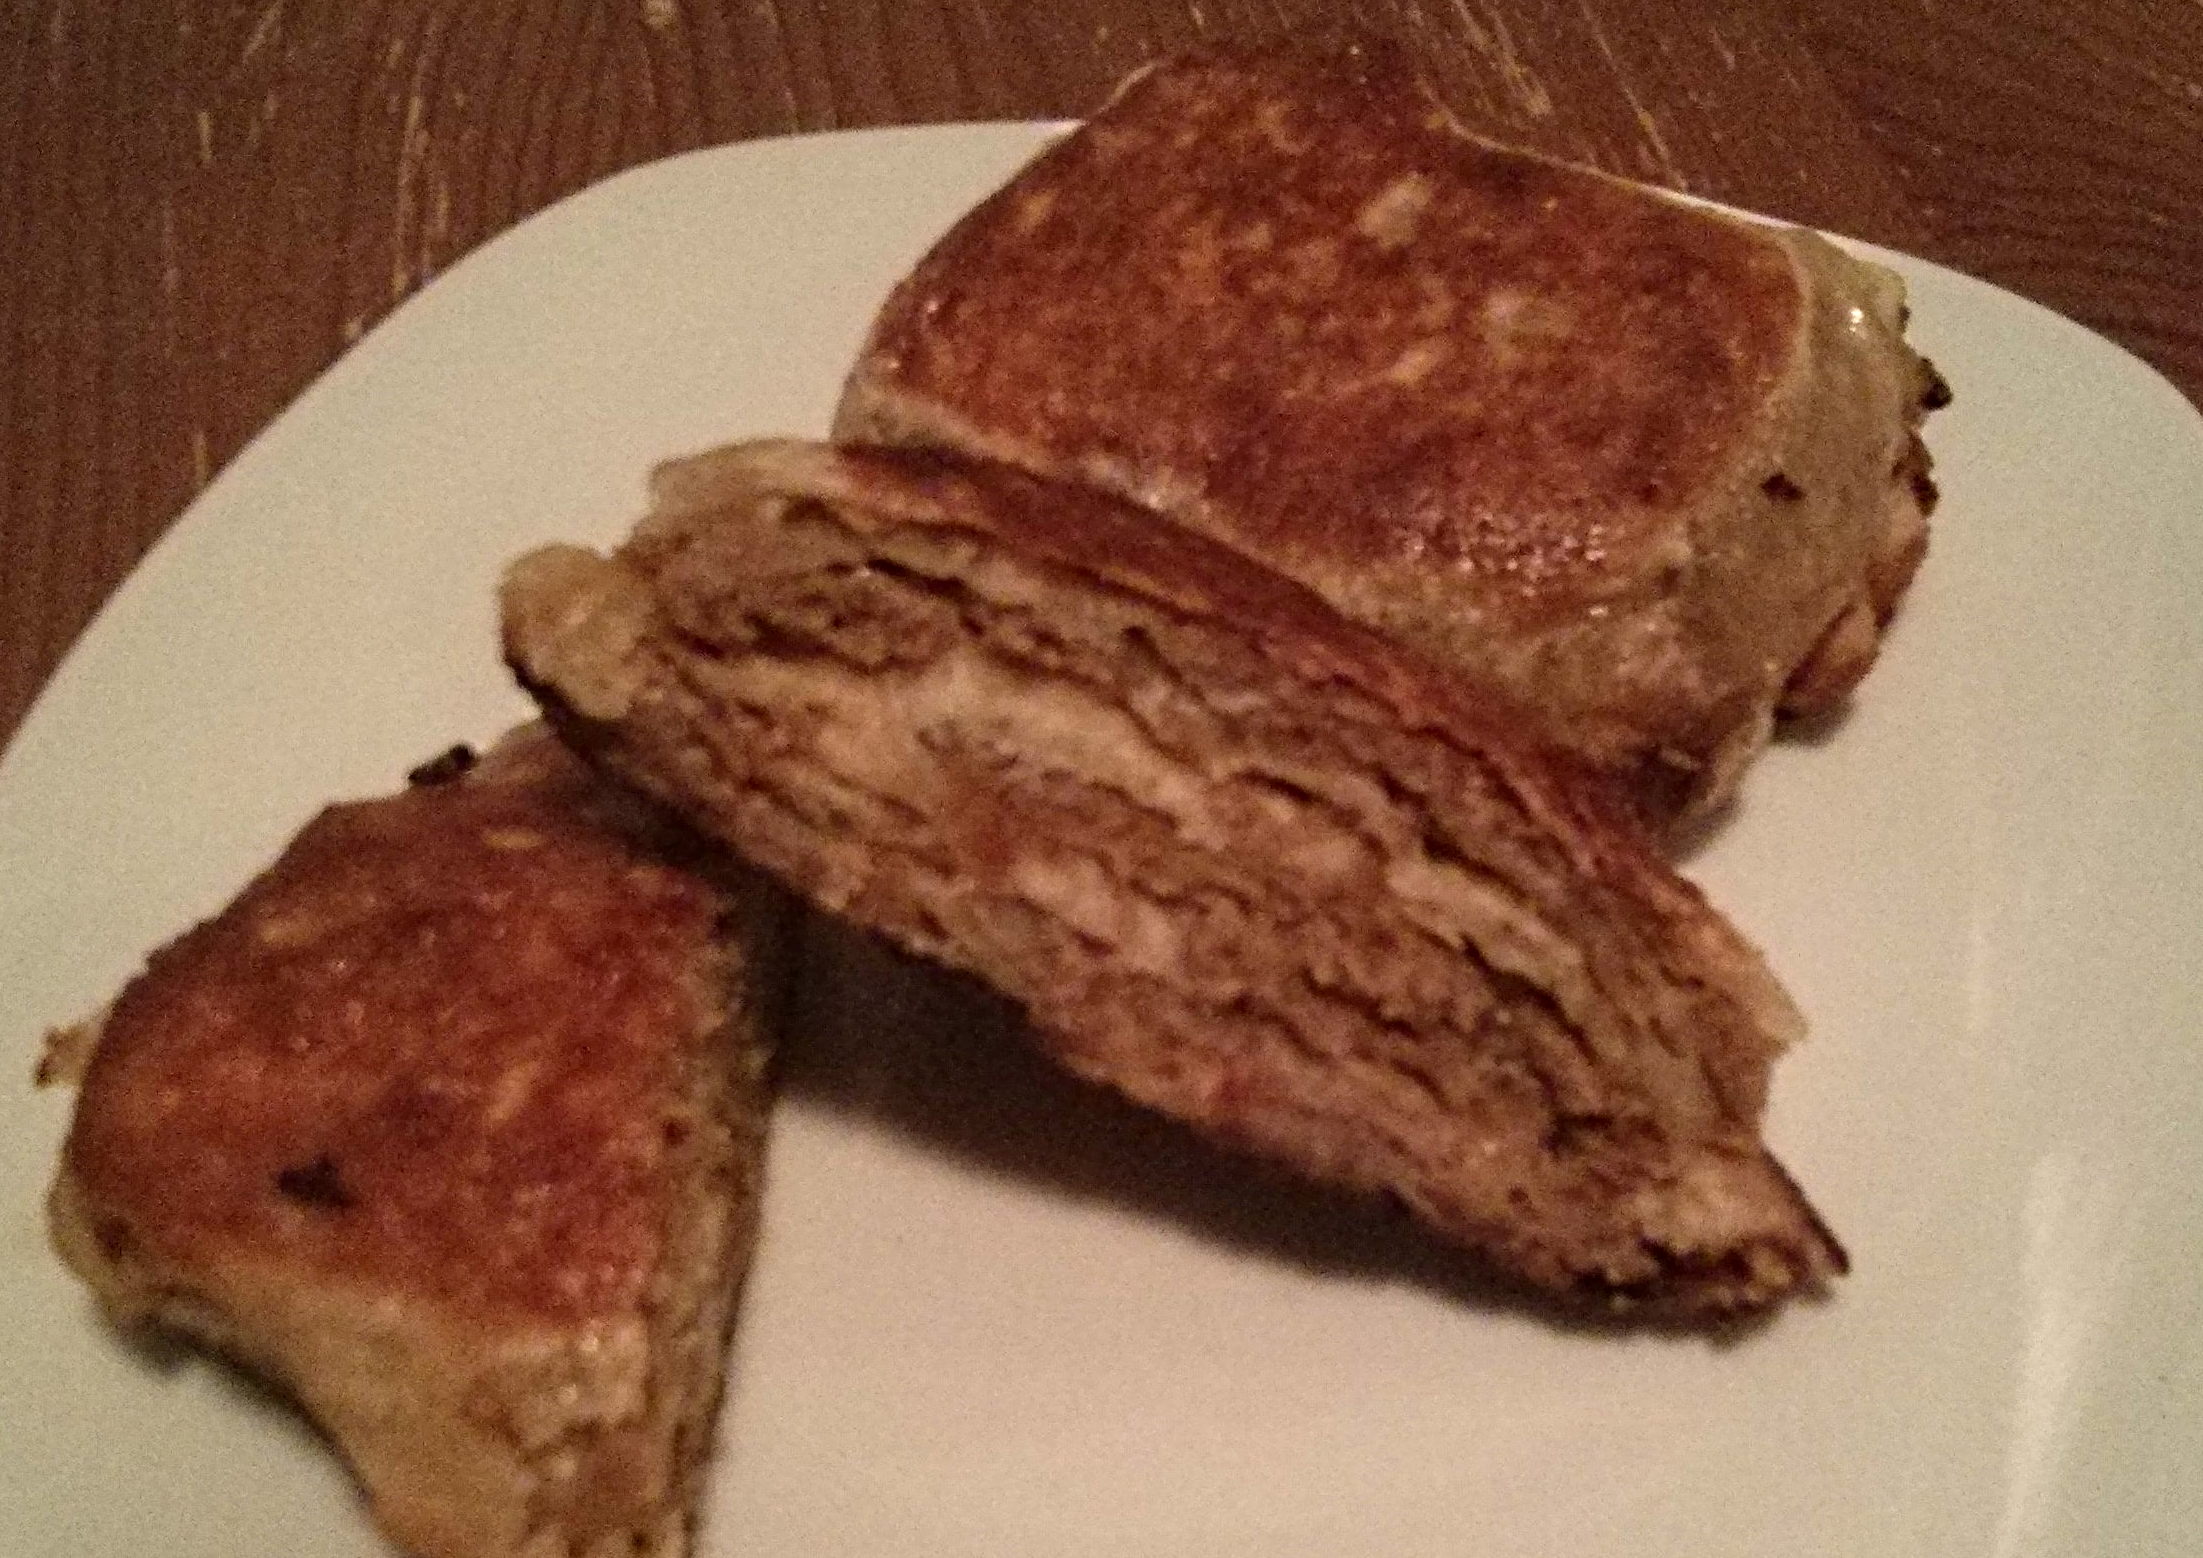
\includegraphics[width=\paperwidth,height=\paperheight]{./bilder/curry-hack-pancakes_ratio.jpg}};

\begin{recipe}[]{Curry-Hack-Pancakes} %Quelle
	\timerecipe[Minuten]{ca. 30+10+30} %mit [EINHEIT]
	\personcount{3} % mit[ART]
	\ingredient{100g Mehl} % ggf. \nicefrac{1}{2}
	\ingredient{1,5 TL Tockenhefe}
	\ingredient{0,75 EL Zucker}
	\ingredient{2 Prisen Salz}
	\ingredient{0,75 EL Sesamöl}
	\ingredient{65ml warmes Wasser}
	\ingredient{1 Ziebel}
	\ingredient{200g Hackfleisch}
	\ingredient{1,5 EL Sojasauce}
	\ingredient{1 EL Worcestersauce}
	\ingredient{1 EL Austernsauce}
	\ingredient{0,25 TL Pfeffer}
	\ingredient{2 TL Currypulver}
	\ingredient{2 EL Speisestärke}

\step
\textbf{100g Mehl}, \textbf{1,5 TL Tockenhefe}, \textbf{0,75 EL Zucker}, \textbf{1 Prisen Salz}, \textbf{0,75 EL Sesamöl} und \textbf{65ml warmes Wasser} zu einem Teig kneten und 30 Minuten ruhen lassen.

\step
\textbf{1 Zwiebel} klein würfeln und in der Pfanne anschwitzen, etwas abkühlen lassen und mit \textbf{200g Hackfleisch}, \textbf{1,5 EL Sojasauce}, \textbf{1 EL Worcestersauce}, \textbf{1 EL Austernsauce}, \textbf{0,25 TL Pfeffer}, \textbf{2 TL Currypulver} und \textbf{2 EL Speisestärke} für die Füllung mischen.

\step
Den Teig in 3 Stücke teilen, jeweils dünn und nahezu rechteckig ausrollen, jeweils gleichmäßig mit Füllung bestreichen. Zum Falten der Taschen das Rechteck zweimal pro langer Seite bis 1/3 der Breite einschneiden. Es sollten neun "gedachte" Quadrate entstehen.

\step
Jetzt jeweils an den Seiten die oberen und unteren Quadrate in die Mitte einklappen. Dann diese Quatrate ganz in die Mitte falten und mit den Klappen von oben und unten einklappen, so dass ein Paket entsteht. Ebenso mit den anderen Teigen verfahren.

\step
Ca. 8 - 10 Minuten mit geschlossenem Deckel auf beiden Seiten goldbraun braten (ca. 4 - 5 Minuten auf jeder Seite).

%\tippbox{\textbf{Tipp:} ...} % Tipp in extra Rahmen
\end{recipe}